\documentclass[a4paper,12pt]{article}

%\usepackage{fontspec}
%\setmainfont{Times New Roman}
\usepackage[scaled=0.92]{helvet}
\usepackage{bbm}
\usepackage{amsfonts}
\usepackage{amsthm}
\usepackage{array}
\usepackage{tabu}
\usepackage{tabularx}
\usepackage[pdftex]{xcolor, graphicx}
\usepackage[utf8]{inputenc}
\usepackage[a4paper, total={6in, 9in}]{geometry}
\usepackage{enumerate}
\usepackage{setspace}
\usepackage{hyperref}
\usepackage{float}
\usepackage{natbib}
\usepackage{amsmath}
\usepackage{ragged2e}
\usepackage{rotating}
\usepackage{chngpage}
\usepackage{bibentry}
\usepackage{commath}
\usepackage{pdflscape}
\usepackage{booktabs}
\usepackage{subcaption}
\usepackage{tikz}
\doublespacing
\hypersetup{colorlinks=true, citecolor=black, urlcolor=blue, linkcolor=black}
\newcolumntype{C}[1]{>{\Centering\arraybackslash}p{#1}}
\geometry{left = 1in, right= 1 in, top= 1 in, bottom=1in}

\setlength\parindent{0pt}

%\date{August, 2019}
\author{Iloanugo Uzoma}
\title{Predicting the Severity of Car Accidents in Seattle}


\begin{document}
\maketitle

\section{Introduction}
The World Health Organization (WHO) reported that about 20 to 50 million people suffer from non-fatal injuries from vehicle accidents globally every year. Some of the risk factors the WHO considers in their report are speeding, driving under the influence of alcohol or other psychoactive substances, improper use of road safety equipment (helmet, seat belts etc.), distracting the driver, unsafe road infrastructure and so on. Also, the Center for Disease Control shows that every year in the United States, about 3 million people are involved in accidents that cause serious injury. In 2017, the cost to the US economy was huge at about \$75billion in medical care cost and lost productivity from vehicle accidents alone. The Seattle Department of Transportation’s annual traffic report shows that there were 10,959 vehicle-related accidents reported by the police in 2017. The effect of car accidents on the society and economy should be of interest to stakeholders and the government.\\

A comprehensive study that measures these risk factors and estimates how they predict the timing of road accidents will be of use to all parties involved. These include private citizens who bear the pain of the accidents; the cooperation and State government that bear the loss in productivity as a result of road accidents; and insurance companies that provide cover for road users. The objective of this project is to fill in the gap. Using data from road accidents in Seattle, we predict road accidents by considering some of the risk factors stated by the WHO and other factors provided by the police data on road accidents. The Washington State Department of Transport (WSDOT) reported that the common cause of accidents specific to Seattle is speeding, intoxication, following cars too closely, defective equipment, poor vehicle maintenance and failure to yield right of way. The dataset we use to create a predictive model should measure these factors to a good extent to enable the algorithm to learn and predict car accidents from the data.

\section{Data}
The data used in the study is from the Seattle Department of Transport (SDOT). The dataset collects information on the event vehicle accidents in Seattle. The information includes the location and other attributes related to the event provided by the Seattle Police Department (SPD). Some attributes that will be considered important for the analysis in the dataset includes – the severity of the accident, location, the number of people involved, number of vehicles, the junction types, under the influence, weather, road condition, light condition, and if the driver was speeding. Other attributes will be considered and the analysis will involve selecting appropriate attributes that best predict the target – the severity of the accident. The target - severity of accident -  and the model will predict the factors that distinguish between a vehicle accident leading to loss of property versus causing serious injuries. The other parts of the research will explore the data and discuss the model most appropriate for the analysis.

\newpage
\section{Methodology}
\textit{Methodology section which represents the main component of the report where you discuss and describe any exploratory data analysis that you did, any inferential statistical testing that you performed, if any, and what machine learnings were used and why.}

\begin{table}[!htbp] \centering \scriptsize
  \caption{Descriptive Statistics}
  \label{}
\begin{tabular}{@{\extracolsep{5pt}}lccccc}
\\[-1.8ex]\hline
\hline \\[-1.8ex]
Total & \multicolumn{1}{c}{N} & \multicolumn{1}{c}{Mean} & \multicolumn{1}{c}{St. Dev.} & \multicolumn{1}{c}{Min} & \multicolumn{1}{c}{Max} \\
\hline \\[-1.8ex]
SEVERITYCODE      &  182660.0 &  0.31 &  0.46 &  0.00 &   1.00 \\
PERSONCOUNT       &  182660.0 &  2.48 &  1.37 &  0.00 &  81.00 \\
VEHCOUNT          &  182660.0 &  1.97 &  0.56 &  0.00 &  12.00 \\
UNDERINFL         &  182660.0 &  0.05 &  0.22 &  0.00 &   1.00 \\
ADDR\_Block        &  182660.0 &  0.65 &  0.48 &  0.00 &   1.00 \\
ADDR\_Intersection &  182660.0 &  0.35 &  0.48 &  0.00 &   1.00 \\
COLLISIONFREQ     &  182660.0 &  0.16 &  0.07 &  0.01 &   0.25 \\
JUNCTION\_FREQ     &  182660.0 &  0.34 &  0.14 &  0.00 &   0.46 \\
WEATHER\_FREQ      &  182660.0 &  0.41 &  0.22 &  0.00 &   0.59 \\
ROAD\_ODDS         &  182660.0 &  0.45 &  0.11 &  0.05 &   0.60 \\
LIGHT\_ODDS        &  182660.0 &  0.45 &  0.11 &  0.05 &   0.57 \\
SPEED\_N           &  182660.0 &  0.95 &  0.22 &  0.00 &   1.00 \\
%SPEED\_Y           &  182660.0 &  0.05 &  0.22 &  0.00 &   1.00 \\
\hline \\[-1.8ex]
\end{tabular}

	\raggedright\footnotesize \justify { \textit{Notes-} The top section is the summary statistics for the whole country, while the bottom is the summary statistics for the only Niger-Delta. The number of violent events in each category is the sum of all entries in the ACLED dataset by LGA year. Figure 2 shows the distribution plot of all violent event and rebel and militia events in the Niger-Delta.}

\end{table}

\begin{figure}[]
	\centering
	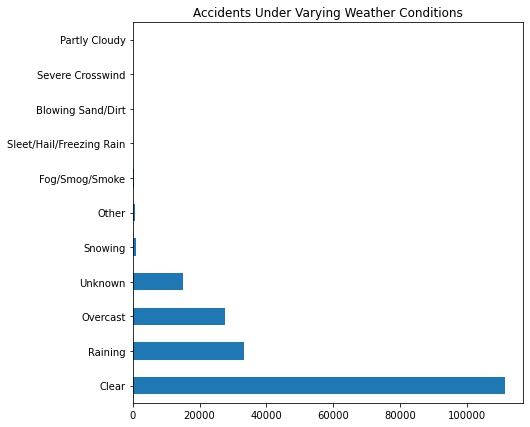
\includegraphics[width=0.8\textwidth]{weather.jpg}
	\caption{Line Plot of}
	\label{fig1}
\end{figure}


\begin{figure}[]
	\centering
	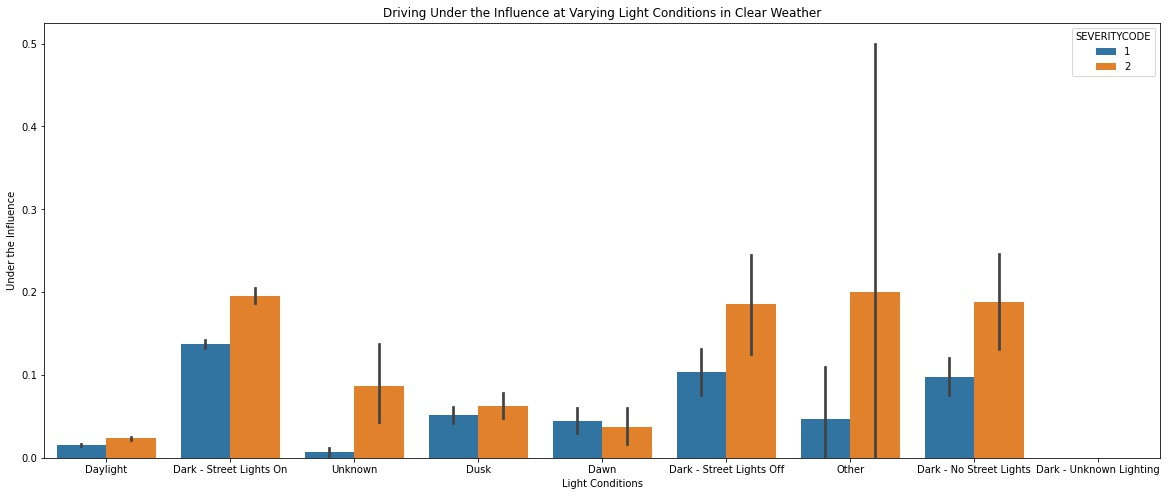
\includegraphics[width=1.0\textwidth]{li_un_wet.jpg}
	\caption{Line Plot of}
	\label{fig1}
\end{figure}

\begin{figure}[]
	\centering
	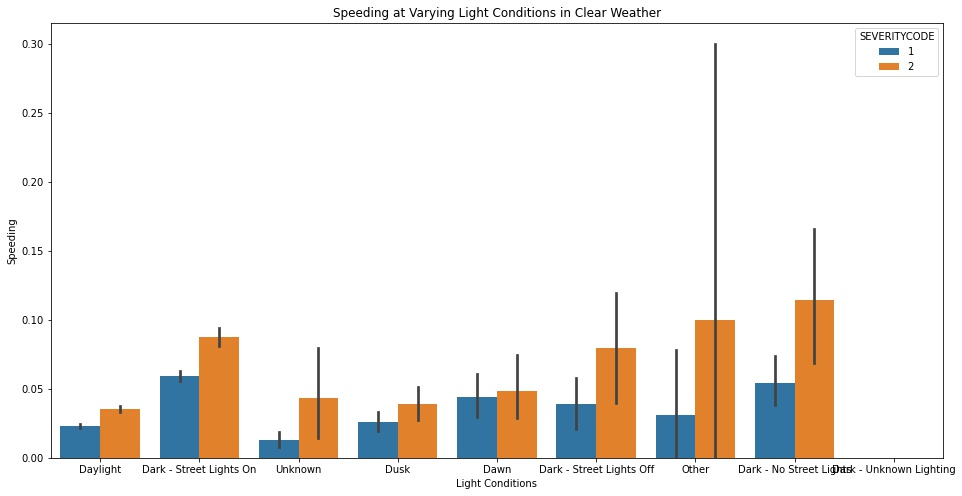
\includegraphics[width=1.0\textwidth]{li_sp_wet.jpg}
	\caption{Line Plot of}
	\label{fig1}
\end{figure}

\begin{figure}[]
	\centering
	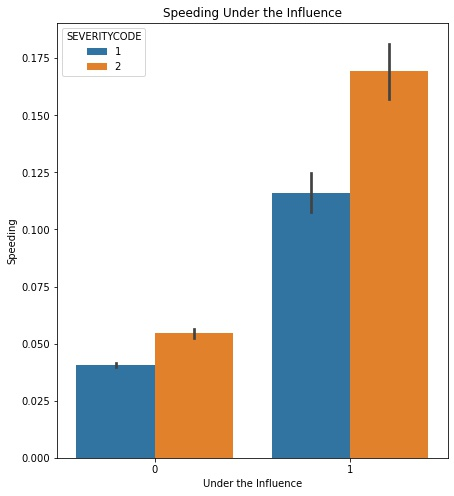
\includegraphics[width=0.6\textwidth]{un_sp_sev.jpg}
	\caption{Line Plot of}
	\label{fig1}
\end{figure}

\begin{figure}[]
	\centering
	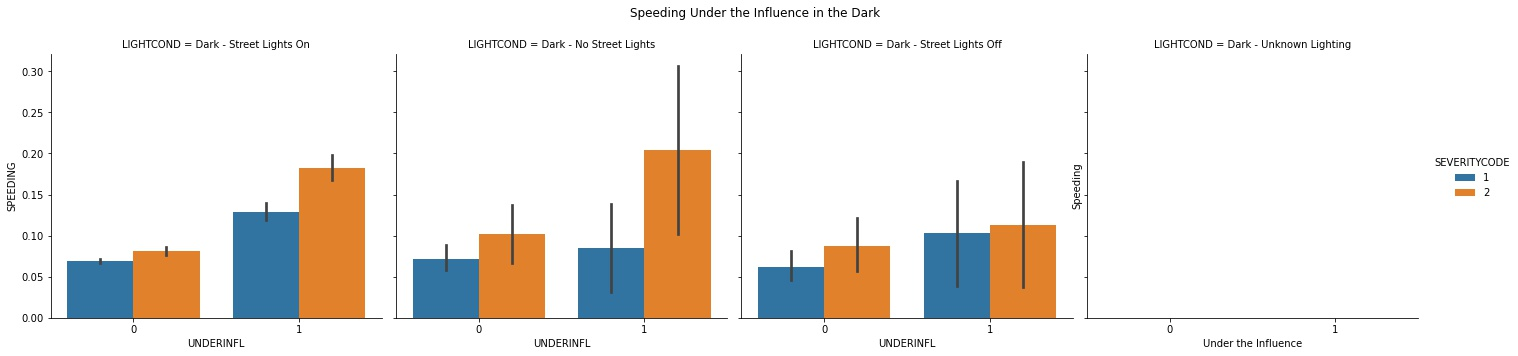
\includegraphics[width=1.0\textwidth]{un_sp_sev_lig.jpg}
	\caption{Line Plot of}
	\label{fig1}
\end{figure}

\begin{figure}[]
	\centering
	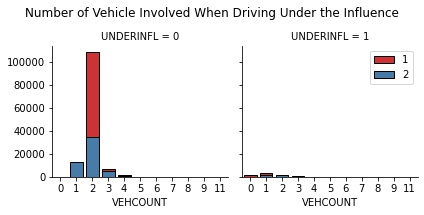
\includegraphics[width=1.0\textwidth]{un_sev_hist.jpg}
	\caption{Line Plot of}
	\label{fig1}
\end{figure}

\begin{figure}[]
	\centering
	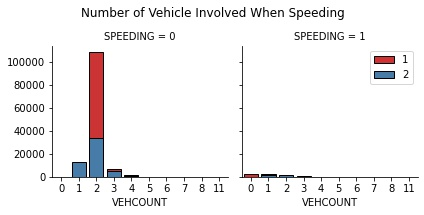
\includegraphics[width=1.0\textwidth]{sp_sev_hist.jpg}
	\caption{Line Plot of}
	\label{fig1}
\end{figure}

\end{document}
